\section{Software}
\label{sec:TeilB_Software}
Um die EDID-Daten in das EEPROM schreiben zu können, muss der Prozessor mit einer gewissen Software programmiert werden. Durch die Verbindung über die USB-Bridge kommuniziert der Prozessor mit dem Computer. Der Datenaustausch arbeitet nach einem definierten Protokoll, auf welches im Softwarekonzept eingegangen wird. Im Anschluss wird die Embedded- sowie die PC-Software mit ihren einzelnen Komponenten beschrieben. 
\subsection{Softwarekonzept}
\label{softwarekonzept}
Um mit dem Prozessor zu kommunizieren, stehen dem PC vier Kommandos zur Verfügung. Diese werden über die Serielle Schnittstelle vom Prozessor empfangen. Die Kommandos folgen dem Format \code{\#Kommando\*}. Sodass ein Kommando definiert von Anfang bis Ende empfangen werden kann, werden die Code-Zeichen \code{\#} und \code{\*} verwendet. Mit dem Zeichen \code{\#} wird dem Prozessor mitgeteilt, dass alle nachfolgenden Zeichen ein Kommando darstellen. Um das Ende des Kommandos mitzuteilen wird das Zeichne \code{\*} gesendet. Wird ein Kommando vollständig empfangen, so wird es interpretiert und die entsprechend Funktion aufgerufen. Nach erfolgreicher Ausführung der entsprechenden Funktion wird ein Return-Wert an den PC gesendet. Die verfügbaren Kommandos um mit dem Prozessor zu kommunizieren und deren Rückgabewerte sind in \reft{tab:avr_commands} beschriebenen.
\begin{table}[h]
\begin{tabular}{|p{6.5cm}|p{2.5cm}|p{3.5cm}|}\hline
\rowcolor{TableBackgroundColor} 
   \textbf{Beschreibung} & \textbf{Kommando} & \textbf{Rückgabewert}	\\ \hline
	Handshake empfangen & \#h* & keiner \\ \hline    
    Start des Schreibvorgangs und setze Adresse im EEPROM auf Null & \#s* & \#1* \\ \hline
    Inkrementiere Adresse im EEPROM und schreibe Daten& \#wX* & \#2* \\ \hline
    Beende Schreibvorgang & \#x* & \#3* \\ \hline
	Prüfsumme angefordert & \#c* & gibt aktuelle Prüfsumme zurück\\ \hline    
    Debug-Ausgabe & \#d* & gibt aktuellen EEPROM-Inhalt zurück\\ \hline
\end{tabular}
\caption{Teil B: Kommandos zum Schreiben des EEPROMs}
\label{tab:avr_commands}
\end{table} \\
Ein Ablaufdiagramm der Funktionalität zum Beschreiben des EEPROMs ist in \refa{fig:ablaufdiagramm_avr} zu sehen. Nach dem Start des Prozessors sendet der ein Handshake \code{h}. Verbindet sich das PC-Prorammm mit der seriellen Schnittstelle und korrekter Baudrate, werden diese Aufforderungen zum Handshake empfangen. Die PC-Software antwortet ebenfalls mit \code{h}, was beiden Teilnehmern die Anwesenheit des anderen bestätigt. Der AVR ist somit Bereit zum Empfangen von Kommandos (siehe \reft{tab:avr_commands}). Um das EEPROM zu beschreiben, wird vom PC das Kommando \code{\#s\*} gesendet, was dem AVR mitteilt, dass im Folgenden Daten zum Beschreiben des EEPROMs gesendet werden. Der PC sendet nun 128 mal das Kommando \code{\#wX\*}, um die 128 Bytes der EDID-Informationen zu senden. Das \code{X} steht für einen Platzhalter und entspricht der Hexadezimalen Schreibweise für binäre Werte von 0 bis 255. Um dem AVR mitzuteilen, dass das Beschreiben des EEPROMs beendet werden und damit keine Daten mehr gesendet werden, wird das Kommando \code{\#x\*} gesendet. Nach jedem empfangenen Kommando sendet der AVR jeweils den Rückgabewert aus \reft{tab:avr_commands} für das entsprechende Kommando. Die PC-Software wartet auf den Empfang des Rückgabewerts und fährt erst nach Erhalt dessen mit dem Schreiben weiterer Kommandos fort. Nachdem alle Bytes in das EEPROM geschrieben sind, fordert das Programm mit \code{\#c\*} die Prüfsumme der EEPROM-Daten an. Dieser Schritt ist notwendig um die Integrität der Daten zu prüfen. Ist bei der Kommunikation ein Fehler unterlaufen, so unterscheiden sich die beiden Prüfsummen von EEPROM und PC-Programm.\\
\begin{figure}[htp]
	\center
	\fbox{	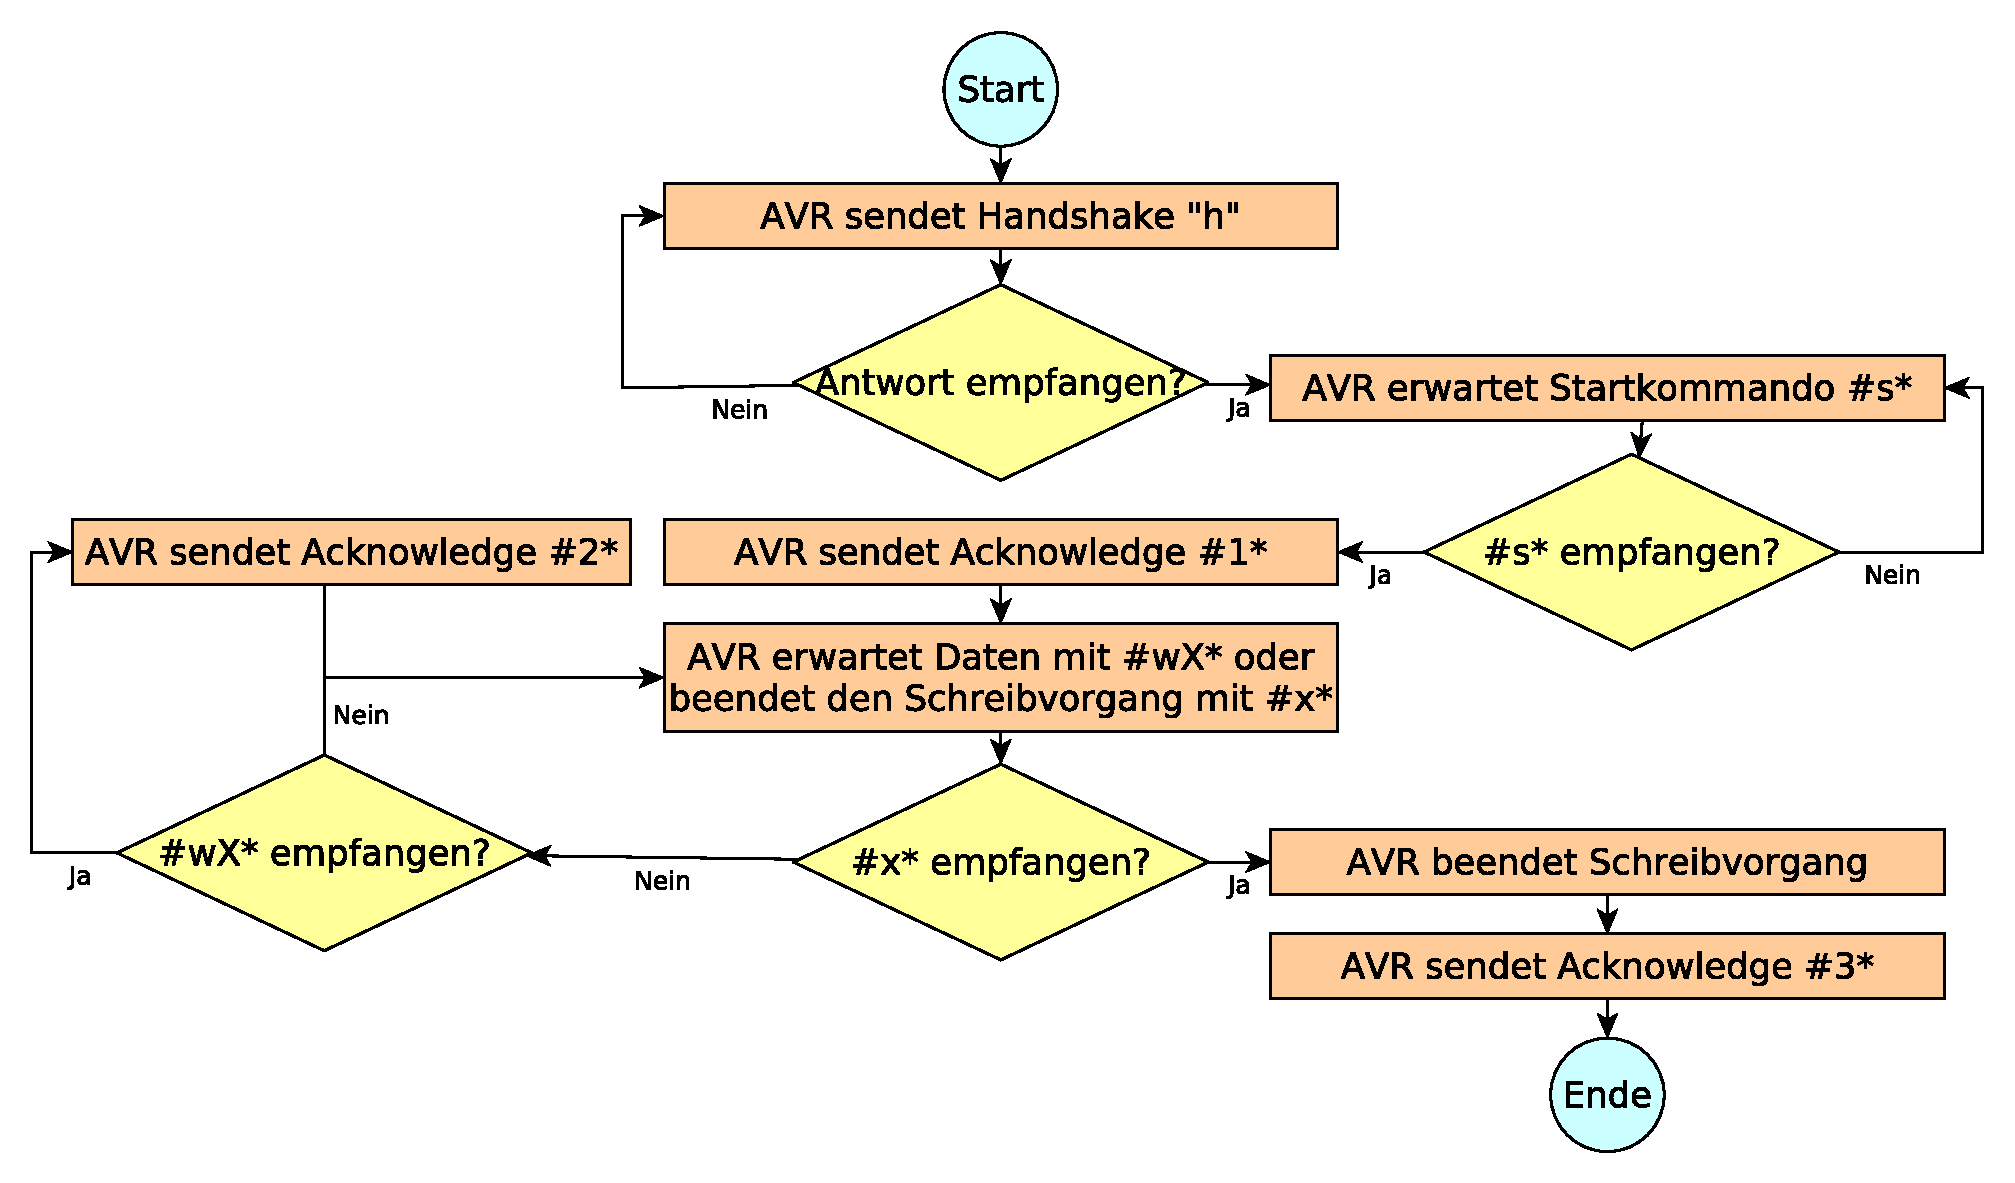
\includegraphics[width=1\textwidth]{TeilB/avr_arch.pdf}}
    \caption{Teil B: Ablaufdiagramme Embedded-Software}
    \label{fig:ablaufdiagramm_avr} 
\end{figure}\\

Für den Fehlerfall, dass die Datenkommunikation abbricht, obwohl bereits das Startkommando \code{\#s\*} gesendet wurde, wird der Zyklus mit jedem erneuten Senden von \code{\#s\*} zurückgesetzt und der Schreibvorgang von vorne begonnen.\\
Wird die PC-Software gestartet und es bleibt das Handshake vom AVR aus (z. B. fehlerhafte oder falsche Software im AVR), so wird innerhalb einer Zeitspanne auf dieses Handshake gewartet und nach Ablauf dieser Zeit abgebrochen und der Fehler angezeigt.\\
Der gesamte Schreibvorgang ist innerhalb einer definierten Zeit abgeschlossen. Tritt im Fehlerfall eine Verzögerung auf, so wird ebenfalls nach Ablauf einer definierten Zeitspanne abgebrochen und der Fehler angezeigt.
\subsection{EDID-Daten auf Embedded-Seite}
In den folgenden Abschnitten wird auf die benötigten Low-Level-Treiber sowie die auf die internen Funktionsweisen der Embedded-Software selbst eingegangen.
\subsubsection{Low-Level-Treiber UART}
Wie bereits in \refc{softwarekonzept} angesprochen werden nach der Interpretation der Kommandos die entsprechenden Funktionen aufgerufen. Der AVR empfängt die Zeichen über die UART-Schnittstelle Zeichen für Zeichen. Wird ein Zeichen empfangen, wird ein Interrupt ausgelöst und dessen ISR\footnote{ISR: Interrupt Service Routine} aufgerufen. Der Quellcode der ISR ist in \refl{lst:uart_isr} gezeigt.
\begin{lstlisting}[%
language=MyC,
caption={Embedded-Software: UART-ISR},
label=lst:uart_isr
]
ISR(USART_RX_vect)
{
   sint8 next_char;
   next_char = UDR0;

   if(next_char == '#')
   {
      uart_str_cnt = 0;
      block_finished = 0;
   }
   if(next_char == '*' && !block_finished)
   {
      block_finished = 1;
      switch(uart_str[1])
      {
      case 's':
         command_ready(CMD_WRITE_START, 0xFF);
         break;
      case 'w':
         command_ready(CMD_WRITE_DATA, uart_str[2]);
         break;
      case 'x':
         command_ready(CMD_WRITE_STOP, 0xFF);
         break;
      case 'd':
         command_ready(CMD_DBG, 0xFF);
         break;
      case 'c':
         command_ready(CMD_CHECKSUM, 0xFF);
         break;
      case 'h':
         handshake_received = 1;
         break;
      default:
         command_ready(CMD_ERROR, 0xFF);
         break;
      }
   }
   if(!block_finished)
   {
      uart_str[uart_str_cnt] = next_char;
      uart_str_cnt++;
   }
}
\end{lstlisting}
Nach dem Empfang eines Zeichens wird dieses in die Variable \code{next_char} gespeichert. Es wird innerhalb einer State-Machine überprüft, ob ein Kommando vollständig mit den Steuerzeichen \code{\#} und \code{\*} empfangen wurde. Solange das Flag \code{block_finished} nicht gesetzt ist, wird das aktuelle Zeichen an einen Buffer \code{uart_str[]} angehängt. Ist das Flag \code{block_finished} gesetzt und das aktuelle Zeichen entspricht \code{\*}, so ist das Kommando bereit interpretiert zu werden. Da das zweite Zeichen des Kommandostrings \code{uart_str[2]} jeweils den eigentlichen Kommandonamen definiert, reicht es diesen auszuwerten und die entsprechende Funktion mit \code{command_ready(uart_i2cCommandType cmd, uint8 data)} anzuspringen.

\begin{lstlisting}[%
language=MyC,
caption={Embedded-Software: Funktionen zum Beschreiben des EEPROMs},
label=lst:eeprom_functions
]
void w_start()
{
   cnt = 0;
   /* Check if an error ocurred during the last transmission and stop i2c connection if true */
   if(connection_status == OPEN)
   {
      connection_status = CLOSED;
   }
   address_counter = 0;
   connection_status = OPEN;    /* Leave connection open */
   _delay_ms(100);
   uart_puts("#1*");
}

void w_data(uint8 data)
{
   cmds[address_counter] = data;
   write_eeprom_byte(address_counter, data);
   address_counter++;
   _delay_ms(100);
   uart_puts("#2*");
}


void w_stop()
{
   address_counter = 0;
   connection_status = CLOSED;
   _delay_ms(100);
   uart_puts("#3*");
   handshake_received = 0;
}

void dbg_output()
{
   uint8 i;
   for(i = 0; i < 128; i++)
   {
      eeprom[i] = read_eeprom_byte(i);
      uart_putc(eeprom[i]);
   }
}

void send_checksum()
{
   uint8 i, byte;
   uint8 timeoutCounter = 0;
   checksum = 0;
   for(i = 0; i < 128; i++)
   {
      eeprom[i] = read_eeprom_byte(i);
      checksum ^= eeprom[i];
   }
   continue_send_Checksum = 1;
   while(continue_send_Checksum == 1 && timeoutCounter < CHECKSUM_TIMEOUT)
   {
      uart_putc(checksum);
      timeoutCounter++;
      _delay_ms(100);
   }
}


\subsubsection{Low-Level-Treiber EEPROM}

\end{lstlisting}

\subsection{EDID-Daten auf PC Seite}
\subsubsection{GTK GUI mit Glade}